\documentclass[a4paper,draft=false]{scrreprt}

\usepackage[utf8]{inputenc}
\usepackage[T1]{fontenc}
\usepackage[english]{babel}

\usepackage{amsmath}
\usepackage{amssymb}

\usepackage{graphicx}

\usepackage{appendix}

%%%%%%%%%%%%%%%%%%%%%%%%%%%%%%%%%%%%%%%%%%%%%%%%%%
% info to go to titlepage
\subject{Case 1}
\title{Damage detection of the Valdemar platform model}
%\subtitle{subtitle}
\author{Kasper Juul Jensen, Lars Roed Ingerslev, Maya Katrin Gussmann}
%\date{\today}

%%%%%%%%%%%%%%%%%%%%%%%%%%%%%%%%%%%%%%%%%%%%%%%%%%
\usepackage{Sweave}
\begin{document}
\Sconcordance{concordance:case1.tex:case1.Rnw:%
1 22 1 1 0 6 1 1 5 3 0 1 1 1 2 1 3 4 0 1 2 54 1}

% Titlepage
\maketitle

% Rnw options need to be set to knitr, not to Sweave!!
% knitr setup:
\begin{Schunk}
\begin{Sinput}
>   # use package knitr and read in used R code,
>   # which is in the file case1.R for better overview
>   require(knitr)
>   read_chunk("case1.R")
>   load("Case1.RData")
>   # preload other packages
>   require(data.table)
\end{Sinput}
\end{Schunk}

Please upload a file \verb+yhat.txt+ containing predictions $\lbrace 0, 1, 2, 3\rbrace$ as one long vector with newline separating the observations. The corresponding order is that given in the \mbox{Cas1\_tst} (Xt), and a small report with a brief introduction/abstract, pre-processing, modeling and model assessment, plus your evaluation of the actual dimensions needed to describe the data/problem.

Please note that the deadline is mid-day.

\chapter{Introduction}

There are three sensors on an offshore platform, that record data for detecting damage to the platform. Damage can occur at three different sites (see table \ref{table:damageclass}) and for three different intensities ($5\%, 10\%, 15\%$). The recorded data is given in the form of Frequency Response Functions (FRFs).

\begin{table}[ht]
\begin{center}
\begin{tabular}{ll}
  \hline
  Class & Description\\\hline
  0 & undamaged\\
  1 & damage in the bottom of the shaft\\
  2 & damage in one of the legs\\
  3 & damage in the top of the shaft\\
  \hline
\end{tabular}
\caption{Damage classes.\label{table:damageclass}}
\end{center}
\end{table}

In this case, $4092$ samples of the three FRFs are given, together with their respective damage classes. The goal is to form a model to predict damage and damage class.

\begin{figure}[hb]
\begin{center}
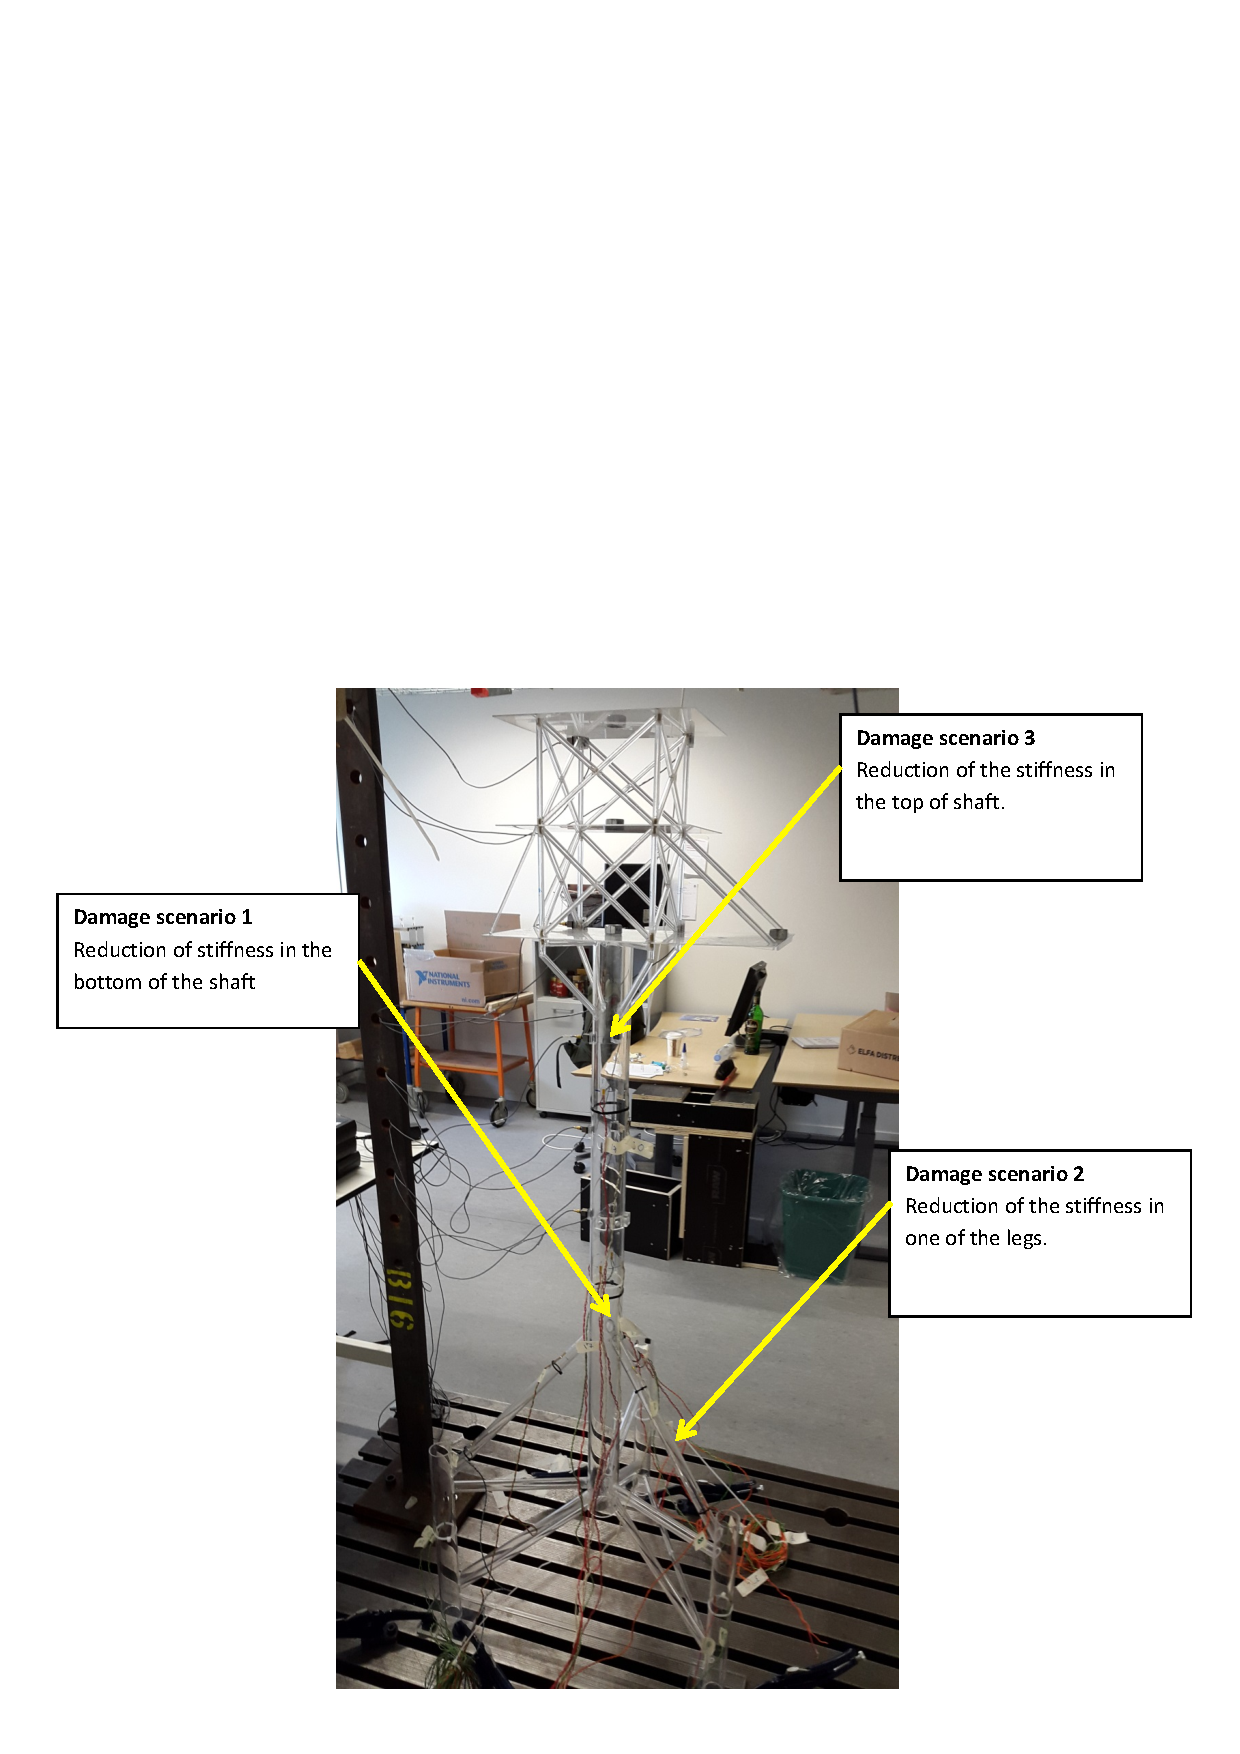
\includegraphics[width=0.7\textwidth]{Valdemarplatform}
\end{center}
\end{figure}

\chapter{Pre-processing}
\section{PLS} % Lars

\chapter{Modeling}
\section{Cross validation \& Majority Vote} % 
\section{KNN} % Kasper
\section{Logistic regression} % Lars
\section{SVM} % Maya
\section{CART} % 



\chapter{Dimensions}

test

%%%%%%%%%%%%%%%%%%%%
%%%%% APPENDIX %%%%%
%%%%%%%%%%%%%%%%%%%%
\appendix
\appendixpage

\end{document}
